% -----------------------------------------------
%   GeoRouting Block
% -----------------------------------------------
\subsection{The GeoRouting Block}
\begin{sloppypar}
The {\em GeoRouting} extension block supports source-routing based on either intermediate geographic waypoints, logical hops (EIDs), or both.  A {\em GeoRouting} block is essentially a list of geo-routing entries, each one specifying an intermediate routing goal. The {\em GeoRouting} block's format is shown in Figure~\ref{fig:georouting-block}; its main part contains only two fields: the flags (which are currently unused) and an entry count that specifies how many geo-routing entries follow.  Each geo-routing entry has several fields.  The flags specify the requirements and contents of the entry. The four flags are:
\begin{description*}
  \item[REQUIRED.] If set, then this entry {\it must} be satisfied for the bundle to be considered delivered.  Otherwise the entry is considered optional.
  \item[ORDERED.] If set, then this entry {\it must} be satisfied before any successive entries can be considered.  Otherwise an intermediate node can pop following entries off the list before this one is satisfied.
  \item[GEO\_PRESENT.] If set, this entry contains a latitude/longitude pair to be used as a routing waypoint.  To satisfy this entry, the bundle must visit a node that is within a specified margin of this coordinate.
  \item[EID\_PRESENT.] If set, this entry contains an EID.  To satisfy this entry, the bundle must, at some point, visit a node whose singleton EID matches the required EID.
\end{description*}
\end{sloppypar}

\begin{figure}
\begin{center}
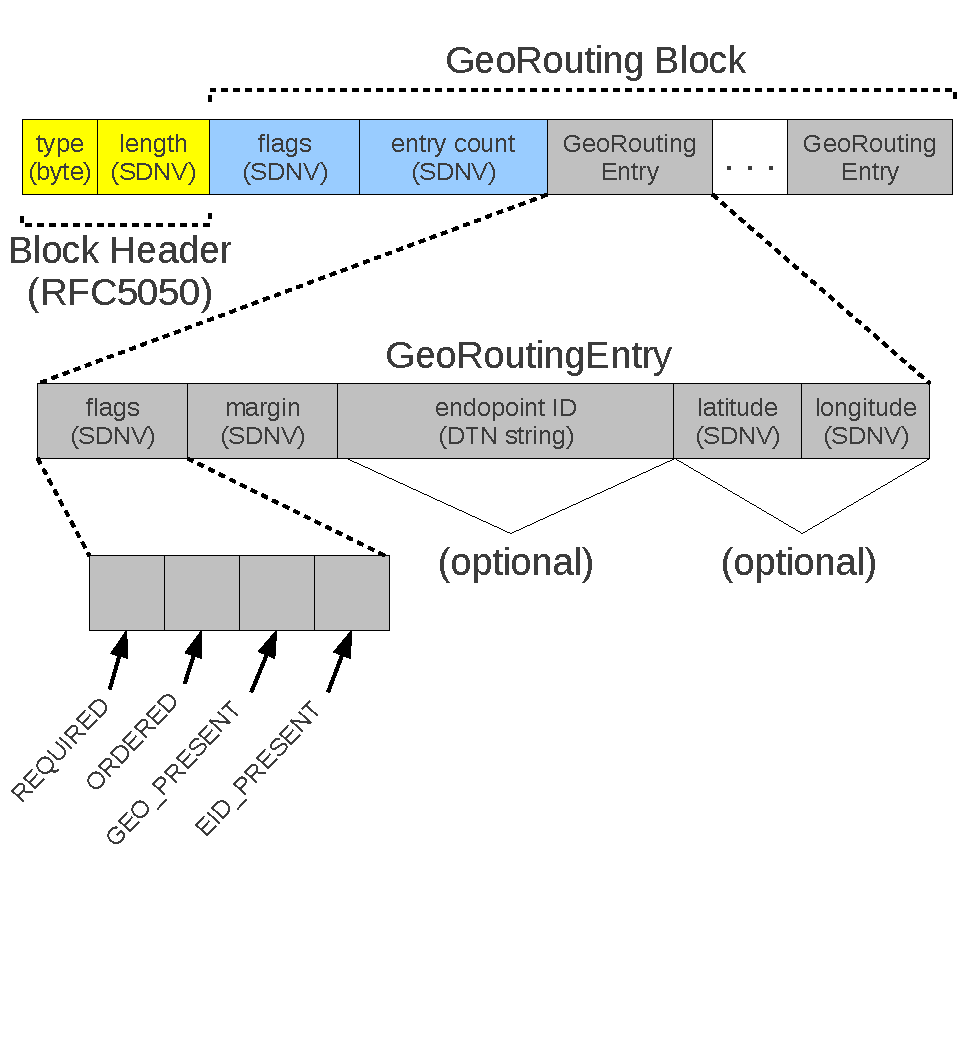
\includegraphics[width=.8\columnwidth]{figures/georouting-block.pdf}
\end{center}
\vspace{-.75cm}
\caption{Format of the GeoRouting Block}
\label{fig:georouting-block}
\vspace{-.5cm}
\end{figure}

If both {\bf GEO\_PRESENT} and {\bf EID\_PRESENT} are set, then the bundle must be carried by the node specified in the EID field to the location specified by the GPS coordinate.  {\bf REQUIRED} and {\bf ORDERED} could be set to false if the sender intends to allow the bundle to take a shortcut if one is available; some entries could be discarded if the bundle finds itself able to skip ahead in the specified geo-trajectory. Our router's use of these fields is described below.

The {\em GeoRouting} block's {\bf margin} specifies {\em how close} the block {\em must} come to any specified coordinate for the entry to be considered satisfied. The margin is a floating point value given in absolute degrees. For example, if $m$ is the margin and $x_0$ and $y_0$ are the required longitude and latitude, then getting the bundle to any point in the range $(x_0\pm m, y_0\pm m)$ will satisfy the entry.  This results in a target area that is roughly rectangular instead of circular, and a particular margin will result in different {\it actual} margins of error at different points on he globe.  This approach keeps the router implementation simple; interpreting the margin as a radius in meters would require more complicated geodetic calculations each time a node's location changes. To represent the margin as an SDNV, we apply the same transformation as with GPS coordinates.

In comparison to the {\em GeoTracking} block, the {\em GeoRouting} block is easier to maintain for the block processor, but more complicated for the routing implementation. The router handles updates to the extension block in the node's data store, and the block processor only needs to serialize the block as it appears, with no modifications.  The details of the router updates are given in the next section. As with the {\em GeoTracking} extension block, we have implemented the {\em GeoRouting} block in both the IBR-DTN core and within the Java API; this allows Java-based applications to create geo-routed bundles directly.


